In this chapter we come to the core of this thesis, namely the empirical performance investigation of the Fribourg construction. We are interested in two things. First, how the different versions of the Fribourg construction compare to each other. That is, how do different combinations of optimisations influence the performance of the construction. Second, we want to know how the Fribourg construction peforms compared to existing complementation constructions. Our main measure for the performance of a construction is the number of states of the produced complement. Throughout this thesis, we will refer to the first question as the \textit{internal} tests, and to the second question as the \textit{external} tests.

To do an empirical performance investigation we need an implementation of the Fribourg construction. We decided to create this implementation in the framework of an existing tool called \goal. This is a Java tool with a graphical user interface for manipulating \om-automata, and it contains implementations of various Büchi complementation constructions. In this way we can easily compare the Fribourg construction to these other construction (see external tests).

The next thing we need for an empirical performance investigation is test data. These are specific sets of automata on which all the tested construction are run. We defined two test sets. The first one, called the \goal{} test set, contains a large number of randomly generated automata. The second one, called the Michel test set, contains just a small number of automata that have a special property.

Having an implementation and test data, the experiments need to be executed. Our chosen implementation approach and test data results in heavy computation tasks, that require a lot of computation power and time. We therefore decided to execute the experiments in a professional high-performance computing (HPC) environment. This environment is the Linux-based HPC computing cluster, called UBELIX, at the University of Bern.\footnote{\url{http://ubelix.unibe.ch}}

In this chapter, we describe each of these points in a separate section. Section~\ref{4_exp_setup} also includes our experimental setup, that is, a listing of the concrete construction versions that we tested, the allocated computing resources, and so on. The results of the experiments will finally be presented in Chapter~\ref{chap_results}.


\section{Implementation}
As mentioned, we implemented the Fribourg consruction as part of the \goal{} tool. This is possible thanks to the extensible plugin architecture of \goal{} which allows to write plugins that contain additional functionality for \goal. Our implementation of the Fribourg construction has therefore the form of a \goal-plugin.

In this section, we first present the \goal{} tool in a general way (Section~\ref{4_goal}). In Section~\ref{4_implementation}, we give some more details about the plugin architecture of \goal, and describe some properties of our implementation. Finally, in Section~\ref{4_verification}, we describe how we verified the correctness of our implementation.


\subsection{GOAL}
\label{4_goal}
\goal{} stands for \textit{Graphical Tool for Omega-Automata and Logics} and is being developed since 2007 by the Department of Information Management at the National Taiwan University (NTU)\footnote{\url{http://exp.management.ntu.edu.tw/en/IM}}. The tool has been presented in various scientific publications~\cite{2007_goal}\cite{2008_goal_ext}\cite{2009_goal}\cite{2013_goal}. The executables of \goal{} can be freely downloaded on \url{http://goal.im.ntu.edu.tw}.

\goal{} allows to graphically and interactively create and manipulate different types of \om-automata, including non-deterministic Büchi automata (NBW). The palette of provided manipulations is vast and ranges from input testing, over conversions to other types of non-deterministic \om-automata, to implementations of graph layout algorithms. Figure~\ref{goal_gui} shows a screenshot of \goal's graphical user interface with an open menu showing the breadth of possible manipulations for \om-automata. 

\begin{figure}[htb!]
\centering
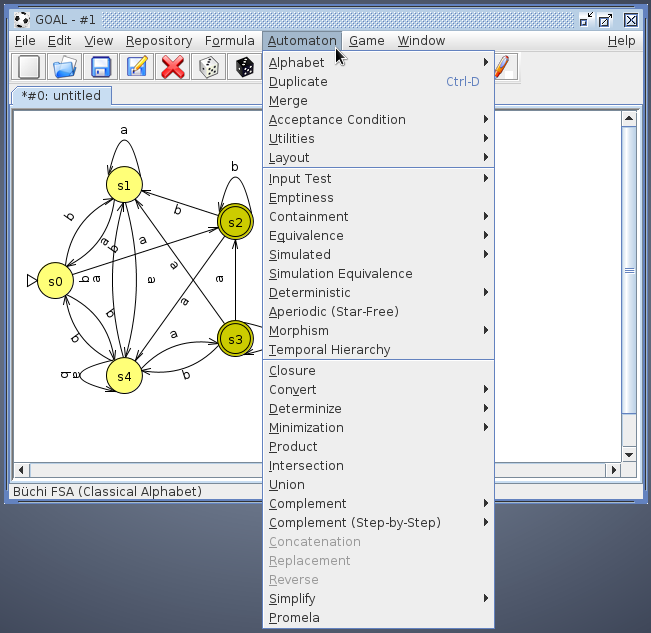
\includegraphics[width=0.4\textwidth]{figures/goal.png}
\caption{The graphical user interface of \goal{} (version 2014--11--17). The open menu item gives an idea about the different types of manipulations that \goal{} provides for \om-automata.}
\label{goal_gui}
\end{figure}

Relevant for our purposes are the complementation constructions for NBW that \goal{} provides. \goal{} comes up with a comprehensive offer in this regard too. In the 2014-11-17 version of \goal{}, there are 10 pre-implemented complementation constructions for NBW. Table~\ref{goal_constructions} summarises these constructions and indicates the authors and the publications on which the implementations are based.

\begin{table}[htb!]
\centering
\begin{tabular}{rlllr}
\hline
\# & Identifier & Name/description & Authors (year) & Ref. \\
\hline
1 & Ramsey & Ramsey-based construction & Sistla, Vardi, Wolper (1987) & \cite{PrasadSistla1987217} \\
2 & Safra & Safra construction & Safra (1988) & \cite{1988_safra_1} \\
3 & ModifiedSafra & Modification by Althoff & Althoff (2006) & \cite{2006_althoff} \\
4 & Piterman & Safra-Piterman construction & Piterman (2007) & \cite{2007_piterman} \\
5 & MS & Muller-Schupp construction & Muller, Schupp (1995) & \cite{Muller199569} \\
6 & Rank & Rank-based construction & Schewe (2009) & \cite{schewe2009buchi} \\
7 & WAPA & Via weak alternating parity automata & Thomas (1999) & \cite{1999_thomas} \\
8 & WAA & Via weak alternating automata & Kupferman, Vardi (2001) & \cite{Kupferman:2001} \\
9 & Slice+P & Slice-based construction (earlier) & Vardi, Wilke (2007) & \cite{vardi2007automata} \\
10 & Slice & Slice-based construction (later) & Kähler, Wilke (2008) & \cite{2008_kaehler} \\
\hline
\end{tabular}
\caption{The pre-implemented NBW complementation constructions in \goal{} (version 2014-11-17).}
\label{goal_constructions}
\end{table}

The construction in Table~\ref{goal_constructions} are sorted by the four fundamental complementation approaches. The first one, Ramsey, is the only construction belonging to the Ramsey-based complementation approach. The following four constructions, Safra, ModifiedSafra, Piterman, and MS, belong to the determinization-based approach. Rank, WAPA, and WAA are representants of the Rank-based approach. Finally, Slice and Slice+P belong to the slice-based approach.

Slice and Slice+P are combined in a single construction in \goal{} but the two specific constructions can be selected by the means of an option. If the P option of Slice is activated, then the Slice+P construction is used, and otherwise the Slice construction is used. In our experiments, we will use the Slice+P version, hoever, we will still refer to this construction as simply Slice in its short form.

Almost the entire functionality of \goal{} is also available via a command line interface. This makes it suitable for automatic batch operation, as it is needed for our experiments. For storing automata, \goal{} defines its own file format called GFF (\goal{} file format) which is based on XML and is typically used with the filename extension \textsf{.gff}.

At this point, it is worth pointing at a related project of the same research group, called the Büchi Store. This is an online repository of classified and tagged \om-automata that can be downloaded in different formats (including GFF). The Büchi Store is located on \url{http://buchi.im.ntu.edu.tw/} and has also been described in a scientific publication~\cite{2011_buchi_store}. Furthermore, there is a binding in \goal{} to the Büchi Store, so that the contents of the store can be directly accessed from \goal{}. For our project we did not make use the Büchi Store, but it is might be an interesting option for related projects.


\subsection{Implementation of the Construction}
\label{4_implementation}
\subsubsection{The Fribourg Construction Plugin}
\goal{} has been designed from the ground up to be modular and extensible. To this end, it has been created with the Java Plugin Framework (JPF)\footnote{\url{http://jpf.sourceforge.net/}}. This framework allows to build applications whose functionality can be easily and seamlessly extended by writing additional plugins for it. These plugins can be installed in the main application without the need to recompile the whole application. Rather, the plugin is compiled separately and the resulting bytecode files are copied to the directory tree of the main application. It is not even necessary to know the source code of the main application in order to write a plugin. The interfaces of JPF itself, and the documentations of the relevant classes of the main application are all that a plugin writer needs to know.

In some more detail, JPF requires an application to define so called \textit{extension points}. For any extension point, multiple \textit{extensions} can be provided. These extensions contain the actual functionality of the application. A JPF application basically consists of extensions that are plugged into their corresponding extension points. A plugin is an arbitrary bundle of extensions and extension points. It is the basic unit of organisation in the Java Plugin Framework.

One of the extension points of \goal{} is called \textsf{ComplementConstruction}. The extensions to \textsf{ComplementConstruction} contain the actual complementation constructions that \goal{} provides. For adding a new complementation construction to \goal, one has thus to ceate a new extension to \textsf{ComplementConstruction}. This extension can then be wrapped in a plugin, and the plugin can be compiled and installed in the main application, what makes it an integral part of it. This means that once the plugin is installed, the new construction is included in \goal{} in the same way as all the other constructions.

This is how we added the Fribourg construction to \goal. The name of our plugin is \textsf{ch.unifr.goal.complement}\footnote{By convention, JPF plugins are named after the base package name of their implementation files.}. It is publicly available and can be installed by anybody in their \goal{} application. We give instructions on how to get, install, and use the plugin in Appendix~\ref{app_plugin}.

In reality, there is more than just the extension point \textsf{ComplementConstruction} that can be extended to add a new complementation construction to \goal. There are separate extension points for, for example, the command line binding, menu inclusion, or step-by-step execution support. We created extensions to all these extension points as well and included them in our plugin. Our aim was to make the integration of the Fribourg construction in \goal{} as complete as possible so that it provides the same facilities as the pre-implemented constructions.

\subsubsection{The Fribourg Construction Options}
In our implementation of the Fribourg construction we also included the three optimisations, R2C, M1, and M2, described in Section~\ref{3_optimisations}. We implemented these optimisation as user-selectable complementation construction options. In the GUI, these options are presented to the user as a list of checkboxes immediately before the start of each complementation task. In the command line mode, there is a command line flag for each option that can be set or not set by the user.

In addition to the three optimisations, we added further options to our construction. Table~\ref{goal_options} lists all the available options for the Fribourg construction. Each option has an identifier consisting of upper-case letters that we will use troughout the rest of this thesis to refer to teh corresponding options.

\begin{table}
\centering
\begin{tabular}{ll}
\hline
Option & Description \\
\hline
R2C & Apply R2C optimisation if input automaton is complete \\
M1 & Apply M1 optmisation (component mergin) \\
M2 & Apply M2 optimisation (colour 2 reduction) \\
C & Make input automaton complete before start of construction \\
R & Remove unreachable and dead states from output automaton \\
RR & Remove unreachable and dead states from input automaton \\
MACC & Maximise accepting states of input automaton \\
B & Use the ``bracket notation'' for state labels \\
\hline
\end{tabular}
\caption{The options of the Fribourg construction in \goal.}
\label{goal_options}
\end{table}

The first three options in Table~\ref{goal_options} represent the three optimisations from Section~\ref{3_optimisations}. The R2C optmisation is implemented so that it applies only to input automata that are complete. That is, selecting R2C for the complementation of an automaton that is not complete has no effect, and the result is the same as if R2C would not have been selected. The options M1 and M2 implement the M1 and M2 optimisations. Since M2 is dependent on M1, it is not possible to select M2 without also selecting M1. This restriction is enforced in both the GUI and the command line interface.

The C option is one of the options that modifies the input automaton before the actual complementation starts. This option first checks if the input automaton is complete\footnote{An automaton is complete if every state has at least one outgoing transition for every symbol of the alphabet.}, and if this is not the case, makes it complete by adding a sink state. This means that an additional non-accepting state, the sink state, is added to the automaton, and from every incomplete state the ``missing'' transitions are added from this state to the sink state. The sink state itself has loop transitions for all symbols of the alphabet.

The purpose of the C option is to be used in conjunction with the R2C optimisation. By making an automaton complete before the start of the construction, we can ensure that the R2C optimisation will be applied. The question then arises whether, in terms of performance, it is worth to do is. Because for making an automaton complete, we have to add an additional state to the automaton what generally increases the complexity of the complementation. This question has been investigated in previous work about the Fribourg construction by Göttel~\cite{2013_bsc_goettel}. In this thesis will re-investigate this point in an extended form.

The R option modifies the output automaton at the end of the construction. In particular, it removes all the so called unreachable and dead states from the complement. Unreachable states are states that cannot be reached from the initial state. Dead states are states from which it is not possible to reach an accepting state. These states can be removed from any automaton without changing the language of the automaton. The pre-implemented complementation constructions Ramsey, Piterman, Rank, and Slice also contain a similar R option.

One usage case of the R option is to determine the number of unreachable and dead state that a complementation construction produces. Complementing the same automaton with and without the R option, and taking the difference of the complement sizes will yield this number. Investigations in this direction have been done with \goal{} by Tsai~et~al.~\cite{2011_tsai}. In our own investigations we will use the R option to determine the number of unreachable and dead states the plain Fribourg construction produces.

The RR option is similar to the R option, except that it removes the unreachable and dead states from the input automaton rather than from the output automaton. This option is a custom creation by us, and the pre-implemented complementation cosntructions in \goal{} do not contain a similar option. We are not using the RR option in our investigations.

The MACC option again modifies the input automaton before the start of the construction. Namely, it applies the technique of the ``maximisation of the accepting set''. This means that as many states as possible are made accepting without changing the language of the automaton. The larger number of accepting state should then simplify the complementation task. This technique has been introduced and empirically investigated by Tsai~et~al. in~~\cite{2011_tsai}. The pre-implemented complementation cosntructions Ramsey, Piterman, Rank, and Slice contain a similar MACC option. In our own investigations we will however not use the MACC option.

Finally, the B option is a pure display option and does not alter the automata or the construction itself. Its effect is to use the bracket notation for state labels, that indicates component colours by different types of brackets, instead of the default notation that uses numbers to specify the component colours.


\subsection{Verification of the Implementation}
\label{4_verification}
% Results on  UBELIX/jobs/2014-11-25
Having an implementation, it is important to verify that it is correct. With correct we mean in this section that the construction produces a valid complement for a given input automaton, that is, that the language of the output automaton is indeed the complement of the language of the input automaton. We verified this point of our implementation as described below. In this sense, we know that our implementation is a valid construction. This is not the same as the verification that our implementation faithfully represents the Fribourg construction as it has been devised by its creators. Rather, this latter point has been informally verified during the whole development period of the implementation, which was possible thanks to the close collaboration with the construction creators.

In order to verify that our implementation produces correct results, we performed so called complementation-equivalence tests in \goal{} against one of the pre-implemented construction. This works as follows. Take an automaton $A$ and complement it with one of the \goal{} constructions. This yields automaton $A^\prime$. Then, complement the same automaton $A$ with our implementation of the Fribourg construction. This yields automaton $A^{\prime\prime}$. Now, by the means of \goal's equivalence operation then test whether $A^\prime$ and $A^{\prime\prime}$ accept the same language.

This approach makes a couple of assumptions. First, it relies on the correctness of the pre-implemented complementation constructions, and on the equivalence operation of \goal{} (which is also based on complementation). Second, with this empirical approach it is of course not possible to conclusively verify the correctness of our implementation. Every passed complemenation-equivalence test just further confirms the hypothesis that our implementation is correct, but it can never be proved. Despite these points, we think that this approach is the best we can do, and that, with a sufficient number of test cases, it can confirm the correctness of our implementation with a high probability.

We tested the Fribourg construction in different versions with all the options that we described in the last section (except the B option as it does not influence the construction). The tested versions are the following.
\begin{itemize}
\item Fribourg
\item Fribourg+R2C+C
\item Fribourg+M1
\item Fribourg+M1+M2
\item Fribourg+R
\item Fribourg+RR
\item Fribourg+MACC
\end{itemize}

We tested each version with 1,000 randomly generated automata. The automata had a size of 4 and an alphabet size between 2 and 4. The pre-implemented construction we tested against, was the Piterman construction. The result was that all the tests were successful, that is, there was not a single counterexample.

With a size of 4, the automata used for the tests are rather small, and it would be interesting to do the tests with bigger automata. However, our limited computing and time resources prevented us from doing so. The equivalence test of \goal{} is implemented as reciprocal containment tests, which include complementation. That is, the overall test includes the complementation of the complements of the test automata. By using bigger test automata, their complements might be already so big that a further complementation is practically infeasible with our available resources. Nevertheless, we think that the high number of performed tests confirms the correctness of our construction with a high probability.


\section{Test Data}
Test data is the sample data that is given to an algorithm as input in order to measure and evaluate certain properties of the output. The test data is an important part of every empirical study and should meet several requirements. It should include enough test cases so that the results are statistically significant. It should not be biased in favour of the tested algorithm. It should cover test scenarios that are relevant for evaluating the performance of the algorithm. Ideally, publicly available test data is used that has also  been used for other empirical studies. In this way, the data is ``objective'' and results of different studies are comparable.

In our case the test data consists of a set of non-deterministic Büchi automata which are provided as input to the Fribourg construction. We chose two different sets of automata of which we believe that together they form a meaningful test set for our study.

The first set of test automata, which we call \goal{} test set, consists of 11,000 NBW of size 15. This test set has been used by a previous empirical study with \goal{} by Tsai~et~al.~\cite{2010_tsai}, and is publicly available. The second set of automata, which we call Michel test set, consists of a family of automata that show a very pronounced state growth for complementation. These automata have been introduced and described by Michel~\cite{michel1988}, hence the name. Below, we describe these two test sets with their relevant properties in separate sections.


\subsection{GOAL Test Set}
\label{4_goal_testset}
The \goal{} test set is the larger and more complex one of the two test sets. In this section, we first introduce the \goal{} test set and describe its basic structure. In the second part, we present the results of an analysis that we did in order to reveal further properties of the \goal{} test set, namely the number and distribution of complete, universal, and empty automata.

\subsubsection{Introduction and Basic Structure}
The \goal{} test set has been created by Tsai~et~al. for an empirical study evaluation the effects of several optmimisations on existing Büchi complementation constructions~\cite{2010_tsai}. This study has been executed in \goal{} and the automata in the test set are available in the \goal{} file format, hence the name \goal{} test set.

The entire test set consists of 11,000 automata of size 15, and 11,000 similar automata of size 20. For our study we used however only the automata of size 15. Hence, when we refer to the \goal{} test set in the rest of this thesis, we specifically mean the 11,000 automata of size 15. The \goal{} test set is publicly available through the following link: \url{https://fribourg.s3.amazonaws.com/testset/goal.zip}\footnote{This link is maintained by the author of the thesis. The original link of the \goal{} tests set that is maintained by the authors of~\cite{2010_tsai} is \url{http://goal.im.ntu.edu.tw/wiki/lib/exe/fetch.php?media=goal:ciaa2010_automata.tar.gz}. This package contains additionally the 11,000 automata of size 20. In the package of the first link, the files have been renamed, however, the content of the files has not been changed.}.

All the automata in the test set have 15 states and an alphabet size of 2. The further properties of the automata, namely accepting states and transitions, are determined by the values of two parameters called \textit{transition density} and \textit{acceptance density}

The transition density determines the number of transitions of an automaton. In some more detail, the transition density $t$ is defined as follows. Let $n$ be the number of states of automaton $A$, and $t$ its transition density. Then $A$ contains $tn$ transitions for each symbol of the alphabet. In the case that $tn$ is not an integer, it is rounded up to the next integer. That is, if one of our automata with 15 states and the alphabet ${0, 1}$ has a transition density of 2, then it contains exactly 30 transtions for symbol $0$ and 30 transitions for symbol $1$. %At creation time the start and end points of these transitions are chosen at random. %Consequently, each state has on average two outgoing and two incoming transitions for each symbol. Therefore, the transition density can also be seen as the average number of outgoing and incoming transitons per alphabet symbol that a state has.

The acceptance density $a$ is defined as the ratio of accepting states to non-accepting states in the automaton. It is thus a number between 0 and 1. If automaton $A$ has $n$ states and an acceptance density of $a$, then it has $an$ accepting states. In the case that $an$ is not an integer, it is rounded up to the next integer. %Which $an$ states are made accepting is determined randomly at creation time.

The \goal{} test set is structured into 110 classes with different transition density/acceptance density pairs. These 110 pairs result from the cartesian product of 11 transition densities and 10 acceptance densities. The concrete transition densities $t^\prime$ and acceptance densities $a^\prime$ are the following:
\begin{align*}
t^\prime & = \left( 1.0,\,1.2,\,1.4,\,1.6,\,1.8,\,2.0,\,2.2,\,2.4,\,2.6,\,2.8,\,3.0 \right) \\
a^\prime & = \left( 0.1,\,0.2,\,0.3,\,0.4,\,0.5,\,0.6,\,0.7,\,0.8,\,0.9,\,1.0 \right)
\end{align*}
Thus, there is one class whose automata have a transition density of 1.0 and an acceptance density of 0.1, another class with a transition density of 1.0 and an acceptance density of 0.2, and so on. Each of the 110 classes contains 100 automata

When Tsai~et~al. created the \goal{} test set, they created the automata within the given constraints of 15 states, an alphabet size of 2, and the appropriate transition densities and acceptance densities at random. According to~\cite{2010_tsai}, they chose this structure and parameter values in order to generate a broad range of complementation problems ranging from easy to hard.


\subsubsection{Further Properties: Completeness, Universality, and Emptiness}

% Format matrices
\renewcommand{\tabcolsep}{0.05cm}
\renewcommand{\arraystretch}{1.05}
\newcolumntype{R}{>{\raggedleft\arraybackslash}p{1.5em}}
\begin{figure}[htb!]
  \centering
  \begin{subfigure}{\textwidth}
    \begin{subtable}{0.47\textwidth}
    % latex table generated in R 3.1.2 by xtable 1.7-4 package
% Sun Aug 16 12:48:04 2015
\begin{tabular}{r|RRRRRRRRRR}
  & 0.1 & 0.2 & 0.3 & 0.4 & 0.5 & 0.6 & 0.7 & 0.8 & 0.9 & 1.0 \\ 
  \hline
1.0 & 0 & 0 & 0 & 0 & 0 & 0 & 0 & 0 & 0 & 0 \\ 
  1.2 & 0 & 0 & 0 & 0 & 0 & 0 & 0 & 0 & 0 & 0 \\ 
  1.4 & 0 & 0 & 0 & 0 & 0 & 0 & 0 & 0 & 0 & 0 \\ 
  1.6 & 0 & 0 & 0 & 0 & 0 & 0 & 0 & 0 & 0 & 0 \\ 
  1.8 & 1 & 1 & 0 & 0 & 0 & 1 & 1 & 1 & 0 & 0 \\ 
  2.0 & 0 & 5 & 1 & 2 & 2 & 3 & 1 & 2 & 2 & 2 \\ 
  2.2 & 5 & 10 & 8 & 5 & 3 & 5 & 8 & 6 & 7 & 1 \\ 
  2.4 & 10 & 6 & 11 & 11 & 8 & 6 & 10 & 20 & 9 & 7 \\ 
  2.6 & 17 & 17 & 12 & 16 & 14 & 19 & 22 & 21 & 19 & 19 \\ 
  2.8 & 27 & 20 & 29 & 32 & 26 & 27 & 30 & 25 & 24 & 19 \\ 
  3.0 & 37 & 37 & 40 & 39 & 34 & 37 & 38 & 35 & 38 & 39 \\ 
  \end{tabular}

    \end{subtable}
    \hfill
    \begin{subfigure}{0.52\textwidth}
    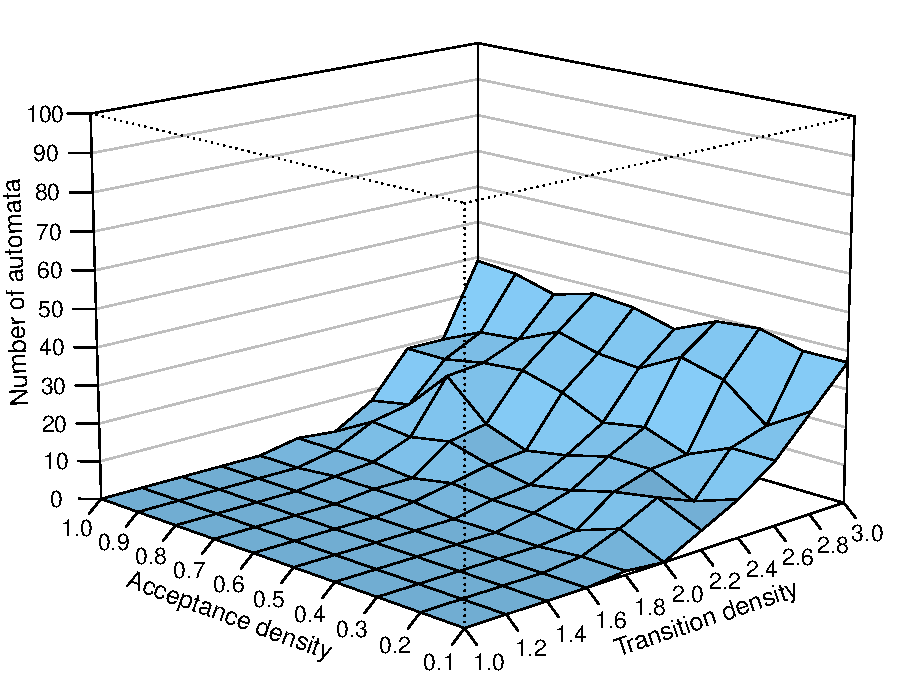
\includegraphics[width=\textwidth]{figures/r/testset/compl.persp.pdf}
    \end{subfigure}
  \caption{Completeness}
  \end{subfigure}

 \begin{subfigure}{\textwidth}
    \begin{subtable}{0.47\textwidth}
    % latex table generated in R 3.1.2 by xtable 1.7-4 package
% Sun Aug 16 12:48:04 2015
\begin{tabular}{r|RRRRRRRRRR}
  & 0.1 & 0.2 & 0.3 & 0.4 & 0.5 & 0.6 & 0.7 & 0.8 & 0.9 & 1.0 \\ 
  \hline
1.0 & 4 & 5 & 5 & 7 & 8 & 4 & 6 & 10 & 4 & 3 \\ 
  1.2 & 1 & 3 & 5 & 8 & 8 & 12 & 10 & 13 & 4 & 14 \\ 
  1.4 & 2 & 17 & 13 & 17 & 20 & 24 & 22 & 21 & 27 & 26 \\ 
  1.6 & 16 & 28 & 30 & 37 & 49 & 42 & 42 & 49 & 45 & 45 \\ 
  1.8 & 31 & 40 & 55 & 59 & 64 & 67 & 76 & 70 & 63 & 78 \\ 
  2.0 & 60 & 64 & 85 & 75 & 83 & 83 & 79 & 90 & 87 & 83 \\ 
  2.2 & 67 & 87 & 86 & 88 & 89 & 91 & 89 & 89 & 89 & 86 \\ 
  2.4 & 88 & 89 & 86 & 92 & 95 & 95 & 94 & 97 & 96 & 97 \\ 
  2.6 & 86 & 93 & 92 & 97 & 97 & 97 & 98 & 96 & 98 & 96 \\ 
  2.8 & 94 & 97 & 95 & 94 & 97 & 99 & 98 & 97 & 97 & 100 \\ 
  3.0 & 99 & 99 & 99 & 97 & 99 & 98 & 100 & 100 & 100 & 99 \\ 
  \end{tabular}

    \end{subtable}
    \hfill
    \begin{subfigure}{0.52\textwidth}
    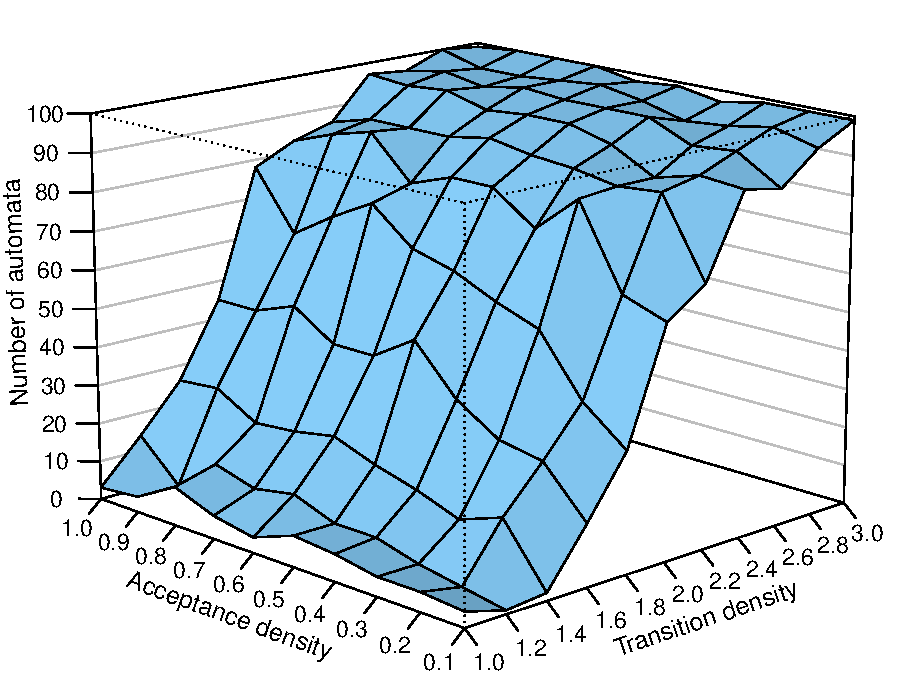
\includegraphics[width=\textwidth]{figures/r/testset/univ.persp.pdf}
    \end{subfigure}
  \caption{Universality}
  \end{subfigure}

  \begin{subfigure}{\textwidth}
    \begin{subtable}{0.47\textwidth}
    % latex table generated in R 3.1.2 by xtable 1.7-4 package
% Sun Aug 16 12:48:05 2015
\begin{tabular}{r|RRRRRRRRRR}
  & 0.1 & 0.2 & 0.3 & 0.4 & 0.5 & 0.6 & 0.7 & 0.8 & 0.9 & 1.0 \\ 
  \hline
1.0 & 17 & 7 & 4 & 5 & 2 & 4 & 3 & 1 & 1 & 0 \\ 
  1.2 & 4 & 2 & 1 & 1 & 0 & 1 & 0 & 0 & 0 & 0 \\ 
  1.4 & 2 & 1 & 0 & 0 & 0 & 0 & 0 & 0 & 1 & 2 \\ 
  1.6 & 0 & 0 & 0 & 0 & 0 & 0 & 1 & 0 & 0 & 0 \\ 
  1.8 & 1 & 0 & 0 & 0 & 1 & 0 & 0 & 0 & 0 & 0 \\ 
  2.0 & 0 & 0 & 0 & 0 & 0 & 0 & 0 & 0 & 0 & 0 \\ 
  2.2 & 0 & 0 & 0 & 0 & 0 & 0 & 0 & 0 & 0 & 0 \\ 
  2.4 & 0 & 0 & 0 & 0 & 0 & 0 & 0 & 0 & 0 & 0 \\ 
  2.6 & 0 & 0 & 0 & 0 & 0 & 0 & 0 & 0 & 0 & 0 \\ 
  2.8 & 0 & 0 & 0 & 0 & 0 & 0 & 0 & 0 & 0 & 0 \\ 
  3.0 & 0 & 0 & 0 & 0 & 0 & 0 & 0 & 0 & 0 & 0 \\ 
  \end{tabular}

    \end{subtable}
    \hfill
    \begin{subfigure}{0.52\textwidth}
    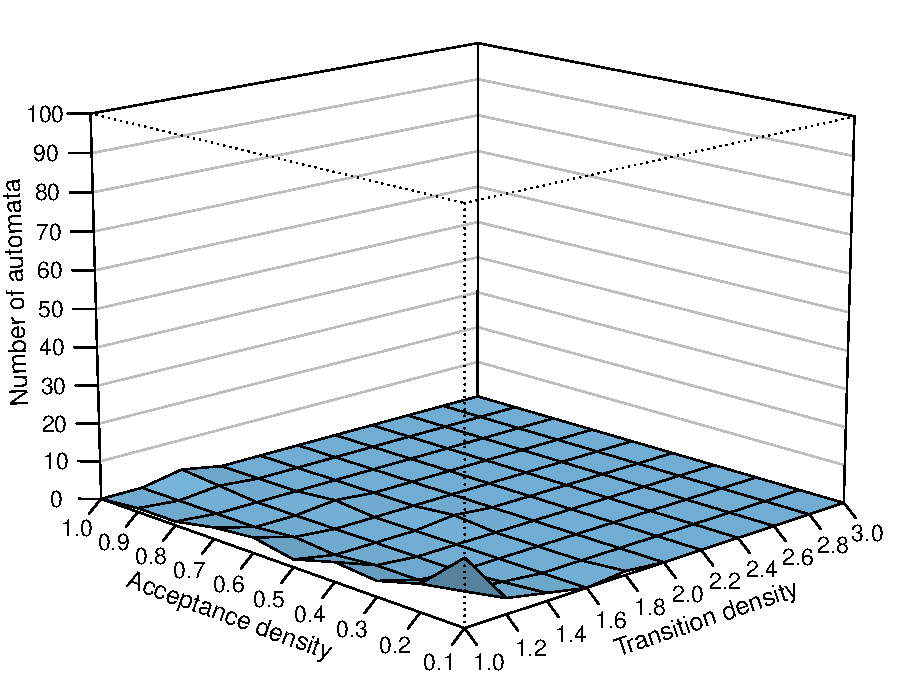
\includegraphics[width=\textwidth]{figures/r/testset/empt.persp.pdf}
    \end{subfigure}
  \caption{Emptiness}
  \end{subfigure}
\caption{Completeness and universality in the GOAL test set.}
\label{4_testset_analysis}
\end{figure}
\tablestyle  % Reset old table style

We analysed some properties of the \goal{} test set that may be of importance for the interpretation of the results of our experiments. In particular, we tested how many automata of the \goal{} test set are \textit{complete}, \textit{universal}, and \textit{empty}.

An automaton is complete if every state has at least one outgoing transition for every symbol of the alphabet. Universality means that an automaton accepts \textit{every} word that can be generated from its alphabet. Emptiness is the contrary of universality and means that an automaton does not accept \textit{any} word (except the empty word $\epsilon$).

To know how many automata are complete is relevant because the R2C optimisation of the Fribourg construction only applies to complete automata. Universality and emptiness are interesting because their respective complement sizes have a lower bound of 1. The complement of a universal automaton is an empty automaton, which can be represented by a single state, and the complement of an empty automaton is a universal automaton which can be represented by a single state as well. In this way we can get an idea of how many unreachable and dead states the Fribourg construction produces. If the produced complement of a universal automata has, say, 2,000 states then 1,999 states of this automata are actually unnecessary as the same automaton could be represented by a single state. We will investigate this aspect to some extent with the R option for the Fribourg construction (see Section~\ref{4_exp_setup}.

\goal{} provides a command for testing emptiness of an automaton. However, it does not provide commands for testing completeness and universality. We therefore implemented these commands on our own as a separate \goal{} plugin (\textsf{ch.unifr.goal.util}, also available as described in Appendix~\ref{app_plugin}). The tests were executed in the execution environment as described in Section~\ref{4_exec_env}. The overall results are as follows.

\begin{itemize}
\item 990 of the 11,000 automata are complete (9\%)
\item 6,796 of the 11,000 automata are universal (61.8\%)
\item 63 of the 11,000 automata are empty (0.6\%)
\end{itemize}

In addition to these overall results, we wanted to know how these properties are distributed over the 110 transition/acceptance density classes. Therefore, we counted the number of complete, universal, and empty automata for each of these 110 classes. This naturally results in three-dimensional data where two dimensions are constituted by the transition density and acceptance density (to form the 110 classes), and the third dimension is the number of automata having a specific property. There are several ways to represent such data, and two of them are matrices and so called perspective plots. In Figure~\ref{4_testset_analysis} we present our results in both of these ways. 

The matrices have 11 rows and 10 columns. The rows represent the transition densities and the columns represent the acceptance densities. The cells represent the measured values for the class constituted by the transition density of its row and the acceptance density of its column. We will use this matrix representation again throughout the rest of this thesis. The perspective plots represent the transition densities, acceptance densities, and measured values along three axes, $x$, $y$, and $z$. The individual data points are connected by lines so that a grid emerges that can be seen to form a three-dimensional surface. Perspective plots can be seen as three-dimensional visualisations of matrices where the cell values extend as ``heights'' along the $z$-axis in the three-dimensional space. However, perspective plots are typically rotated, and this rotation is chosen for making the presented data optimally visible. In Figure~\ref{4_testset_analysis}, looking at the perspective plots is like looking at the corresponding matrices from the upper left corner. We will use perspective plots throughout the rest of this thesis. While their relation to matrices is the same, their rotation will be different. For example, in Chapter~\ref{chap_results}, the viewpoint of the perspective plots will correspond to looking from the bottom right corner at the corresponding matrices.

Regarding the data itself, we can identify the following points. With 9\%, a relatively small number of the automata is complete. This affects the R2C optimisation, which therefore makes a difference to only 9\% of the test data, while leaving 91\% unaffected. We can see that there are no complete automata in classes with transition densities up to 1.6, and then starting from 1.8 the number starts to increase up to a ratio of 34--40\% at a transition density of 3.0. Naturally, a higher number of transitions in the automata increases the probability that each state has at least one outgoing transition for every symbol of the alphabet. Considering that a transition density of, for example, 3.0 means that each state has on average three outgoing transitions for every symbol of the alphabet, this ratios might seem rather small. However, a single incomplete state is enough to make the whole automaton incomplete, even though all the other states would be complete. With a total number of 15 states, the probability of an incomplete state is apparently still quite high, even for a transition density of 3.0, as our empirical data suggests. Naturally, the acceptance density does not influcence the ratio of complete automata.

The ratios look very different for universality. With 61.8\%, a very high number of automata in the test set is universal. This high number might result from the small alphabet of just two symbols of the test automata. With a smaller alphabet, there are fewer possible words, and thus a higher probability that an automaton accepts all the possible words. It would be interesting to investigate the universality ratio of similar automata with larger alphabet sizes. As for completeness, the ratio of universal automata also increases with the transition density, although much faster up to a ratio of 100\%. In addition, we can see a slightly higher number of universal automata in classes with higher acceptance densities (although the pattern is clearly dominated by the transition density). We can summarise this, by saying that more transitions and more accepting states increase the probability that a given word is accepted, and thus the probability that an automaton accepts all the possible words.

The other extreme is the percentage of empty automata, which is just 0.6\%, or 63 instances. Apparently the probability that an automaton of size 15 and with 15 to 45 transitions per alphabet symbol accepts no words at all is very small. The probability is highest in automata with low transition densities and acceptance densities. 


\subsection{Michel Test Set}
Our second test set is very different from the first one. It consists of few well-defined, rather than a large number of random automata. These automata are the Michel automata with $m=\{1,\dots,4\}$, that we call Michel 1, Michel 2, Michel 3, and Michel 4, respectively.

Michel automata have been introduced in 1988 by Max Michel in order to prove a lower bound for the state growth of Büchi complementation of $(n-2)!$, where $n$ is the number of states of the input automaton~\cite{michel1988}\cite{1996_thomas}. Michel constructed a family of automata, characterised by the parameter $m$, that have $m+1$ alphabet symbols, and $m+2$ states. He proved that the complements of these automata cannot have less than $m!$ states. Since the number of states of the input automata is $n = m + 2$, the state growth in terms of input and output states is $(n-2)!$, which is around $(0.36n)^n$.

Michel automata are thus very hard automata, and that is why we chose them as our second test set. By testing our Fribourg construction on very hard automata, we can empirically determine ``lower bounds for the lower bounds'' for the state complexity of our construction. For example, if in our experiments we observe a state growth of a Michel automaton of, say, $(0.99n)^n$, then the real (theoretical) lower bound of the construction is either $(0.99n)^n$ or higher. But it cannot be less than $(0.99n)^n$, because with our experiment we have a proof that there exists an automaton on which our construction produces a state growth of $(0.99n)^n$.

Michel automata are very hard to complement, but of course we cannot prove that they are the \textit{hardest} ones (of their respective size) for our construction. If for example, the Michel automaton with six states (Michel 4), produces a state growth of $(0.99n)^n$, then we don't know if this is the hardest automaton of size 6 for our construction (in which case the real state complexity of our construction would be $(0.99n)^n$), or if there is another automaton of size 6 that produces an even larger complement (in which case the real state complexity of our construction would be higher than $(0.99n)^n$). However, since Michel automata are so hard, we think that they give a useful approximation of a state complexity lower bound of our construction.

In Figure~\ref{4_michel_automata} we present the four Michel automata with $m=\{1,\dots,4\}$, as they are defined in~\cite{michel1988} and~\cite{1996_thomas}. They are in particular:
\begin{itemize}
\item Michel 1: 3 states, 2 symbols,  7 transitions
\item Michel 2: 4 states, 3 symbols, 14 transitions
\item Michel 3: 5 states, 4 symbols, 23 transitions
\item Michel 4: 6 states, 5 symbols, 34 transitions
\end{itemize}

All Michel automata have a single accepting state. The reason that we included only the first four Michel automata are of practical nature. Michel automata are so hard, that starting from Michel 5, the required computing and time resources are so high, that it would become practically infeasible for us to carry out the complementation process. We present some extrapolations on this topic when we discuss the results of the Michel experiments in Chapter~\ref{chap_results}.

\newcommand{\subwidth}{0.42}
\begin{figure}[htb!]
\centering
  \begin{subfigure}[t]{\subwidth\textwidth}
  \MichelOne
  \caption{Michel 1 ($m=1$)}
  \end{subfigure}
  \begin{subfigure}[t]{\subwidth\textwidth}
  \MichelTwo
  \caption{Michel 2 ($m=2$)}
  \end{subfigure}

  \begin{subfigure}[b]{\subwidth\textwidth}
  \MichelThree
  \caption{Michel 3 ($m=3$)}
  \end{subfigure}
  \begin{subfigure}[b]{\subwidth\textwidth}
  \MichelFour
  \caption{Michel 4 ($m=4)$}
  \end{subfigure}
\caption{The Michel automata with $m = \{1,\dots,4\}$, an alphabet size of $m+1$, and $m+2$ states.}
\label{4_michel_automata}
\end{figure}


\section{Experimental Setup}
\label{4_exp_setup}

\subsection{Internal Tests}
\label{4_internal}
In the internal tests our aim is to compare different versions of the Fribourg construction. A specific version of the Fribourg construction is composed of a combination of options. Options can be the 

As presented in Section~\ref{optimisations}, there are three optimisations to the Fribourg construction:
\begin{itemize}
\item R2C: if the input automaton is complete, remove all states whose rightmost colour is 2
\item M1: merge certain adjacent sets within a state
\item M2: reduce 2-coloured sets (requires M1)
\end{itemize}

Furthermore, our GOAL plugin includes, among others, the following options:
\begin{itemize}
\item C: make the input automaton complete (by adding a sink state)
\item R: remove unreachable and dead states from the output automaton
\end{itemize}

The versions of the Fribourg construction that we chose for our internal tests consist of combinations of these five options. According to the nature of the two test sets (the GOAL test set and the Michel automata), we chose two different sets of versions for the two test sets. We are now first going to describe the setup for the GOAL test set and then the one for the Michel test set.


\subsubsection{GOAL Test Set}

For the tests on the GOAL test set, we chose the following eight versions of the Fribourg construction:
\begin{enumerate}
\item Fribourg
\item Fribourg+R2C
\item Fribourg+R2C+C
\item Fribourg+M1
\item Fribourg+M1+M2
\item Fribourg+M1+R2C
\item Fribourg+M1+R2C+C
\item Fribourg+R
\end{enumerate}

The first version is the plain Fribourg construction without any optimisations or options. The next two versions are devoted to investigate the R2C optimisation. Version 2 applies the optimsation only to the automata which happen to be complete (and as we have seen in Section~\ref{goal_testset} these are 9\%). Version 3, on the other hand, makes all input automata preliminarily complete by adding a sink state, so that the R2C optimisation can be applied to \textit{all} automata. The question here is, does it pay off to increase the size of the automata by one (for adding the sink state) but then being able to apply R2C, or is it better to not add the extra state but then not applying R2C neither?

Similar investigations about the R2C optimisation of the Fribourg construction have been made by Göttel~\cite{2013_bsc_goettel}. In particular, he compared Version 1 in our above listing with Version 3. His results were that the mean complement sizes of Version 3 are higher than in Version 1. He evaluated, however, only the mean values, but looking closely at the results suggests that the median values could be in favour of Version 3. Therefore, we decided to reinvestigate this question. Indeed, in our own results the median complement sizes of Version 3 are considerably lower than the ones of Version 1 and Version 2. We will further elaborate on this point in Chapter~\ref{chap_results}.

Versions 4 and 5 in our above listing are for investigating the M1 and M2 optimisations. As M2 requires M1, there are only these two possible combinations. Versions 6 and 7 then enhance the ``better'' one of Version 4 and 5 with R2C and its alternative R2C+C. As we will see in Chapter~\ref{chap_results}, the better one of Version 4 and 5 in terms of median complement sizes is Version 4. That is, the application of M2 results in a decline, rather than a gain, in performance compared to the application of M1 alone. We have to note at this point that such results are always specific to the used the test set, and not universally valid. With a different test set, Version 5 might indeed be better than Version 4. As we will see in the next section, this is the case for our alternative test set consisting of the first four Michel automata.

Version 8, finally, is again the plain Fribourg construction, but this time the output automata are reduced by removing their unreachable and dead states. Comparing the results of Version 8 with Version 1 gives an idea of how many unreachable and dead states the Fribourg construction produces. This is inspired by the paper of the GOAL authors~\cite{2011_tsai} in which the number of unreachable and dead states is one of the main metrics for assessing the performance of a construction.

% As in Section~\ref{optimisations}, we refer to the first optimisation as R2C, the second one as M1, and the third one as M2. These optimisations have the following dependencies:
% \begin{enumerate}
% \item R2C can only be applied if the input automaton is complete
% \item M2 can only be applied if M1 is also applied
% \end{enumerate}

% Regarding the dependency of R2C, there are two possibilities. First (\em{R2C-A}), the R2C optimisation is selectively applied to the input automata which are complete, and not to the others. Second (\em{R2C-B}), all automata are made complete beforehand (by adding a sink state), and then the R2C optimisation is applied to all the automata.

% Göttel ~\cite{2013_bsc_goettel} has compared \em{R2C-B} to a plain version of the Fribourg construction where no optimisations at all are applied. He used the same test data as we do. The result was that \em{R2C-B} produces on average slightly less states, but the peak number of generated states are higher than in the plain version. It will be interesting to see if we can replicate these results, and how the selective application of the R2C optimisation (\em{R2C-A}) performs compared to \em{R2C-B}.

% Regarding the dependencies of the M1 and M2 optimisation, there are only two cases we can test. First, M1 alone, and second, M1 and M2 together. Assuming that the R2C optimisation adds a certain performance gain on top of an existing construction, we can then combine the better one of \em{M1} and \em{M1+M2} with R2C. We can already reveal at this point that \em{M1} performs slightly better than \em{M1+M2} on our test set, even though \em{M1+M2} has a better theoretical worst-case complexity. This topic is further discussed in Chapter~\ref{chap_results}. Thus, the version that we will want to test is \em{M1+R2C}.

% Furthermore, we can also investigate the effect of some generic optimisations on our construction. The most generic optimisations, which are included in most complementation constructions in GOAL, and also our plugin with the Fribourg construction, are:
% \begin{enumerate}
% \item Maximise the acceptance set of the input automaton (MACC)
% \item Remove unreachable and dead states from the output automaton (R)
% \end{enumerate}

% By applying these two optimisations to the best version of the Fribourg construction, we can see how far we can go with tweaking our construction, with respect to our set of test automata.

% Summarising, for the internal tests we are going to carry out runs of the following versions of the Fribourg construction:
% \begin{enumerate}
% \item \em{Fribourg}
% \item \em{Fribourg+R2C}
% \item \em{Fribourg+R2C+C}
% \item \em{Fribourg+M1}
% \item \em{Fribourg+M1+M2}
% \item \em{Fribourg+M1+R2C}
% \item \em{Fribourg+M1+R2C+MACC+R}
% \end{enumerate}

\subsubsection{Michel Test Set}
The versions we tested for the Michel test set are the following:
\begin{enumerate}
\item Fribourg
\item Fribourg+R2C
\item Fribourg+M1
\item Fribourg+M1+M2
\item Fribourg+M1+M2+R2C
\item Fribourg+R
\end{enumerate}

The rationale for choosing these versions is basically the same as for the GOAL test set with the following differences. First, Michel automata are complete, thus it is not necessary to apply the C option. Rather, R2C will automatically apply to all automata. Second, the aim of Version 5 is again to enhance the better one of Versions 3 and 4 with R2C. However, contrarily to the \goal{} test set Fribourg+M1+M2 is better than Fribourg+M1 for the Michel automata. That is why Version 5 is Fribourg+M1+M2+R2C.


\subsection{External Tests}
In the so called external tests we compare the best version of the Fribourg construction with different complementation constructions, again for both the GOAL test set and the Michel test set. The concrete constructions we compared for the external tests are the following.

\begin{enumerate}
\item Piterman+EQ+RO
\item Slice+P+RO+MADJ+EG
\item Rank+TR+RO
\item Fribourg+M1+R2C (\goal{} test set) and Fribourg+M1+M2+R2C (Michel test set)
\end{enumerate}

For the alternative constructions, we chose the Piterman, Slice, and Rank construction. These constructions are representative for three of the four main complementation approaches, determinization-based, slice-based, and rank-based. The fourth complementation approach is Ramsey-based and there is an implementation of the Ramsey construction in \goal{}. However, in preliminary tests, we realised that this construction is not performant enough to be used on our test sets within our time and memory constraints. The authors of \goal{} came to a similar conclusion when they made similar experiments on the \goal{} test set~\cite{2011_tsai}. In their case, the Ramsey construction could not complete any of the 11,000 automata within the set time and memory constraints, and they went on to do the result analysis without the Ramysey construction.

The same applies to all the other constructions that are implemented in \goal{}. We did preliminary tests with all of them and saw that only the three mentioned constructions, Piterman, Slice, and Rank, can be resonably used on the \goal{} test set\footnote{The Safra construction would also have been possible, but the Safra construction is similar to the Piterman construction.}.

The three chosen constructions also have optimisations in their implementations in \goal{}. To have a fair comparison to the best version of the Fribourg construction, which also uses optimisations, we activated the optimisation of these constructions as well. In particular, we chose those optimisations which are set as default in the \goal{} GUI for each construction.

We use Fribourg+M1+R2C for the \goal{} test set and Fribourg+M1+M2+R2C for the Michel test set. This is because these two versions are the most performant ones for the respective test sets.


% \textbf{Justification why to use only piterman, slice, and rank}$\\$
% Notes in UBELIX/jobs/2014-10-09: $\\$
% Made test with complementing the first 10 of the size 15 test set with all constructions, and only piterman, slice, and rank (and safra) completed all of them. $\\$
% See Tsai (2011)~\cite{2011_tsai} page 5: they compared ramsey, piterman, rank, and slice. But ramsey couldn't complement any of the 11,000 automata of size 15. $\\$
% Ramsey, piterman, rank, and slice are representative for the four main complementatio approaches: Ramsey-based, determinization-based, rank-based, and slice-based.


\subsection{Time and Memory Limits}
We defined a time limit of 600 seconds CPU time and a memory limit of 1 GB per complementation task in the GOAL test set. That means, if the complementation of a single automaton is not finished after 600 seconds CPU time or uses more than 1 GB memory, the task is aborted and marked as a \textit{timeout} or \textit{memory excess}.

These limits correspond to the ones used by the experiments of the \goal{} authors~\cite{2011_tsai}. However, from their paper it is not clear if their time limit is in CPU time or wallclock time. But since they used different computing nodes, our results regarding the number of timeouts will anyway differ from theirs.

The reason for these limits is simply the restricted amount of time and memory resources that we have available for the experiments. In an ideal world, we would let every complementation task run to its end, no matter how long it takes and how much memory it uses. This would give a perfectly unbiased picture of the results. By setting time and memory limits, we basically exclude the most difficult automata from the experiment. However, as mentioned, the practical reasons of limited time and computing power force as to make this compromise.

The timeout and memory limit of 1 GB apply just to the automata of the \goal{} test set. For the Michel test set we did not set a timeout because we wanted each one of the four automata to finish. The longest complementation task of a Michel automaton consequently durated 109,810 seconds which is about 28 hours. We set a very high memory limit of 14 GB for the Michel test set to avoid memory excesses as we wanted each automaton to successfully complete. The number of 14 GB is determined by the physically available memory on the used computing nodes. All Michel automata successfully completed with this amount of memory.

The timeout was implemented by the means of the \textsf{ulimit} Bash builtin\footnote{\url{http://linux.die.net/man/1/bash}}, which allows to set a maximum time after which running processes are killed. The memory limit was implemented by setting the maximum size of the Java heap, which can be done by the \textsf{-Xmx} option to the Java Virtual Machine (JVM). The heap is the main memory area of Java and the place where all the objects reside. Note that since our memory limit defines actually the size of the Java heap, the total amount of memory used by the process is higher than our limit, as Java has some other memory areas, for example for the JVM itself. However, this is a rather constant amount of memory and independent from the current automaton, so it does not disturb the relative comparisons of the results.

The presence of aborted complementation task require the consideration of the so called effective samples in the result analysis, as introduced in the experiment paper of the \goal{} authors. The effective samples are those automata which have been successfully completed by \textit{all} constructions that are to be compared to each other. Imagine two constructions $A$ and $B$ where $A$ is successful complementing all the automata, whereas $B$ has timeouts or memory excesses at 100 of the automata. If we would now take, for example, the median complement sizes of the two result sets without first extracting the effective samples, then $B$ is likely be assessed as too good relative to $A$, because $B$'s results do not include the 100 automata at which it failed, and which are thus likely to have large complement sizes with $B$. The same 100 automata would however be included in the results of $A$. Therefore, all the result analysis of the experiments with the \goal{} test sets, that we present in Chapter~\ref{chap_results}, are based on the effective samples of the result sets. 


\subsection{Execution Environment}
\label{4_exec_env}
We executed the experiments on a high performance computing (HPC) computer cluster called UBELIX at the University of Bern\footnote{\url{http://ubelix.unibe.ch}}. This cluster consists of different types of Linux-driven HPC computing nodes, and is managed by Oracle Grid Engine\footnote{\url{http://www.oracle.com/us/products/tools/oracle-grid-engine-075549.html}} (formerly known as Sun Grid Engine) version 6.2. Oracle Grid Engine is a so called load scheduler that is responsible for automatically distributing computing tasks to computing nodes.

The basic workflow of working on the cluster is to prepare a so called job and specify the resources that the job requires for running (time, memory, number of CPU cores, and so on). Then the job can be submitted to the grid engine. The grid engine first puts incoming jobs in a queue and then automatically dispatches them to suitable computing nodes as soon as the required capacity is available.

A job in our case is the execution of a construction (or version of the Fribourg construction) over an entire test set. Thus, we were running 22 jobs in total. We arranged that all jobs were run on identical nodes with the following specifications:

\begin{itemize}
\item Processor: Intel Xeon E5-2665 2.40GHz (64 bit)
\item CPU cores: 16
\item Operating System: Red Hat Enterprise Linux 6.6
\end{itemize}

Since we use the execution time (CPU time) as a secondary metrics, next to the complement sizes, it is important that all complementation tasks are executed on the same type of hardware. \goal{} is multithreaded and thus the jobs may use multiple CPU cores. The number of CPU cores a job may use is not restricted (up to the number of available cores on the node, in our case 16), but our observation is that the jobs use a rather small number of cores (2--3). Note that the measurement of the execution time is not affected by the number of cores a process uses, as the CPU times are measured separately on each core and then added together.  

% \begin{itemize}
% \item mpi.q
%   \begin{itemize}
%   \item hnode 01--42
%   \item Intel Xeon E5-2665 2.40GHz
%   \item 16 CPU cores (slots)
%   \item 64 GB RAM
%   \item $\rightarrow$ 4 GB RAM per core (slot)
%   \item h\_cpu limit: 72:00:00
%   \item h\_rt limit: 73:00:00
%   \end{itemize}
% \item highmem.q
%   \begin{itemize}
%   \item jnode 01--21
%   \item Intel Xeon E5-2665 2.40GHz
%   \item 16 CPU cores (slots)
%   \item 256 GB RAM
%   \item $\rightarrow$ 16 GB RAM per core (slot)
%   \end{itemize}
% \end{itemize}


% \begin{enumerate}
% \item Internal on GOAL testset
% \item External on GOAL testset
% \item Internal on Michel automata
% \item External on Michel automata
% \item Completeness of GOAL testset
% \item Universality of GOAL testset
% \end{enumerate}

% The tests are successful with the following resources:

% \begin{tabular}{|p{1.5cm}|l|r|r|r|r|r|p{3.5cm}|}
% \hline
% Test & Queue & Slots & \parbox[t]{1.75cm}{Job\\memory\\limit} & \parbox[t]{1.75cm}{Job CPU\\time limit} & \parbox[t]{1.75cm}{CPU time\\limit per\\automaton\\} & \parbox[t]{1.75cm}{Memory\\limit per\\automaton\\} & Notes \\
% \hline
% 1 and 2 & mpi.q & 4 & 4 GB & 72:00:00 & 600 sec. & 1 GB & rank -tr -ro has to be run on 10 partitions of the test set \\
% \hline
% 3 and 4 & highmem.q & 4 & 16 GB & 72:00:00 & None & 14 GB & piterman -eq -sim -ro out of memory on Michel N4 \\
% \hline
% 4 & mpi.q & 4 & 4 GB & 72:00:00 & None & 1 GB & \\
% \hline
% 5 & mpi.q & 4 & 4 GB & 72:00:00 & None & 2 GB & universal -m piterman -eq -ro \\
% \hline
% \end{tabular}
